\documentclass{kththesis}
\usepackage[hidelinks]{hyperref}
\usepackage{array}
\usepackage{float}
\usepackage[parfill]{parskip}

\usepackage[acronym]{glossaries}
\usepackage[titletoc]{appendix}

\makeglossaries
\newacronym{di}{DI}{Deionized}
\newacronym{diw}{DIW}{Deionized water}
\newacronym{ftir}{FTIR}{Fourier transform infrared spectroscopy}
\newacronym{nmr}{NMR}{Nuclear magnetic resonance spectroscopy}
\newacronym{ic}{IC}{Ion chromatography}
\newacronym{cmc}{CMC}{Carboxymethylcellulose sodium salt}
\newacronym{dmso}{DMSO}{Dimethyl sulfoxide-D6}
\newacronym{mwco}{MWCOk}{Molecular weight cut off}
\newacronym{M}{M}{Molar}

% % colors (bajs)
% \pagecolor{black}
% \color{green}
%
\usepackage{csquotes} % Recommended by biblatex
\usepackage[style=ieee,sorting=none,backend=biber]{biblatex}
\urlstyle{same}
\addbibresource{references.bib} % The file containing our references, in BibTeX format

% numeric
\setlength{\parindent}{0pt}

% \bachelortrue

\title{This is a new title!!!}
\alttitle{Alt title}
\author{Hjalmar Jakobsson}
\email{hjahja@kth.se}
\supervisor{Andre Holzapfel}
\examiner{Roberto Bresin}
\programme{Media programmf}
\school{com sci}
\date{\today}

% Uncomment the next line to include cover generated at https://intra.kth.se/kth-cover?l=en
\kthcover{kth-cover.pdf}


\begin{document}

% Frontmatter includes the titlepage, abstracts and table-of-contents
% \frontmatter

\includepdf[pages=1]{kth-cover.pdf}
\pagenumbering{roman}

% \titlepage

\begin{abstract}
This is the abstract

\end{abstract}

\begin{otherlanguage}{swedish}
  \begin{abstract}
    Detta är det svenska abstractet.

  \end{abstract}
\end{otherlanguage}

% Print the glossary
\printglossary[type=\acronymtype,nonumberlist]

\tableofcontents
\let\cleardoublepage\clearpage
% Mainmatter is where the actual contents of the thesis goes
\mainmatter

\chapter{Introduction}

\section{Background}
One of the most important aspects of training for musicians are their ears. A musicians job is to deal with the auditory perception, and in vernacular english improving one's auditory perception is commonly referred to as ear training. However, ear training can be broken down into many different categories of perceptual training, some of which are very important to continually practice for musicians and others who are less important.
One important aspect of ear training to musicians is relative interval identification. When musicians practice relative interval identification, the goal is to learn how to recall and identify different musical intervals. In western tonal harmony there are 12 notes and hence there are also only 12 different musical intervals. On a keyboard each interval can be produced, eg. by playing a low C note on a piano and then play each note of the octave simultaneously with it until you reach the C one octave above. If you continue above C one octave above, you will perceive the same intervals all over again untill you reach the next C octave. This phenomenon is called categorical perception. Categorical perception (CP) is a mechanism whereby non-identical stimuli that have the same underlying meaning become invariantly represented in the brain \cite{klein2011role}.

Relative interval identification is one aspect of auditory perception that is a categorical perception and the goal of the present study is to evaluate two different interactive methods for training relative pitch identification on the set of western tonal musical intervals, i.e. the notes of the piano.
One of the methods tested is based on how relative interval training is implemented in most cases on many popular mobile applications in the iOS app store. The second method is a new method designed under the hypothesis of being a more musical procedure for training relative intervals than the conventional method, and even more important is the fact that this new method gives the user ability to discriminate more and more intervals per unit time as their ability improves in contrast to the traditional modality where there is a limit to how fast users can play the game and improve themselves.

Many interactive tools for improving relative interval identification are based on the same interactive protocol.

- List of tried and tested applications during the research phase. goodEar Pro; Relative Pitch Interval Ear Training, Interval Ear Training, Piano Ear Training, Ear Trainer, Ear Beater

Initially, two notes are played back to the user that together form a musical interval. Then it is upon the user of the application to input to the application which interval the user identifies it as. If the interval is identifies correctly, there is an enforced pause before the next set of two notes forming a new interval are played back. This procedure can be summarized as a question, an answer, and then the enforced pause (QAP).
The length of the pause varies between applications but is usually around 1 second; in some applications its shorter and others a few tenths of milliseconds longer.
This pause is interesting because the length of the pause lies within a temporal range that is close to the pace at which musical intervals can be played in a song or melody. This suggests that removing the pause and playing back the next question instant/aneously upon answering could make training more similar to a real musical context and not just viewed as a musical training tool.
Within all the applications tested each interval played back is also separate from the previously played interval. Every time the user answers correctly two new notes are played back and each consecutive pair of notes represent one single interval and there is no relation from one question to the next. However, this has just happened to become just a convention but there is nothing that restricts one from making each question dependent on the previous one and by doing so making the exercise protocol more similar to how real melodies are played. This is how the second method works, from here on referred to as connected intervals (as opposed to traditional separated intervals).
Connected intervals is a protocol for categorical learning and identification of musical intervals. Each training session is initialized with two notes played back representing one interval. After the identification of this initial interval the next note is played back instantaneously upon correct user input of the first interval. Identification of the next interval is now done by comparing each consecutive note to he previous one by holding the previous note in short-term memory. Hence, only single notes are played back at each iteration of the game session after the initial two-note interval. This allows for the user to dictate the pace at which the training is done dynamically and it allows for training at very high speed should the user be very good at identifying intervals. Symbolically the protocol can be presented as follows: playback notes AB, input AB —> playback note C, input BC —> playback note D, input CD, and so on.

\section{Theory}

todo... ???

\chapter{Related Work}
% Term’s to research: intra-parietal-sulcus; superior temporal gyrus; hippocampus; rostral anterior cingulate cortex; so that these can be explained. w/refs

\section{Auditory perception / neurology}

There are multiple aspects to auditory perception and each aspect of auditory perception is thought to be correlated with distinct areas in the brain.
In the late 1970s two classical studies were made suggesting that humans process musical intervals in a categorical fashion. In 1978 XXX conducted a study on melodic intervals showing that musical intervals were perceived categorically by trained musicians \cite{burns1978categorical}. XXX did experiments in 1979 showing that "a phenomenon similar to categorical perception of speech sounds exists for perception of simultaneous musical intervals. That is to say, trained musicians have internalized the concepts of major and minor third to such an extent that sounds they can label differently are more discriminable than sounds given the same name." \cite{zatorre1979identification}
In following decades highly refined tools, such as brain scanning and the fMRI scannner, was invented which has resulted in many studies related to music and perception having been conducted within the community of neuroscience, some of which are presented in the following paragraphs
XXX found that "pitch identification is distinguishable from pitch discrimination on the base of activation in the IPS. IPS activity during pitch identification may be the auditory counterpart of numerosity encoding in the visual domain." \cite{schwenzer2011numeric}.

IPS had previously been shown to be actived, by XXX, during visual tests of  numerosity processing activated the intraparietal sulcus (IPS) \cite{castelli2006discrete}.
Pitch contour perception led to higher activity in the right superior temporal gyrus as compared to all other auditory tests (violet). The contour is the direction of change - the up or down movement of pitch which is regarded as one of the most salient features of relative pitch.
Pitch contour perception and discrimination activated the hippocampus and the rostral anterior cingulate cortex stronger than pitch identification. Pitch contour perception activated the right superior temporal gyrus stronger than pitch identification and tone localization.
In short their pitch identification test measured identification of a single freq amongst a set of four; During pitch contour perception, the participants were to detect whether or not a pitch ascended within a melody of descending pitches; In the localization task, the investigator instructed the participants to indicate the presentation side of the higher tones (918 Hz) as compared to the lower tones (900 Hz) on a pair of headphones.
For testing pitch discrimination, participants compared two successive tones in each trial. Pitch discrimination is the ability to discriminate between small differences in pitch or JND (just noticeable differance) \cite{schwenzer2011numeric}
XXX found in a very recent study published in 2019 that musicians with absolute pitch showed increased activitity in the planum temporale, which they think may reflect the matching of pitch information with internal templates \cite{leipold2019absolute}.
Todo: look into how planum temporale is located in relation to the rSTS. Would CP processing occur in a similar template matching fashion as with absolute pitch?
In 2013 XXX conducted a study looking at auditory short term memory (ASTM) with the aim to find out what activitie can be seen when humans actively try to retain tones in memory and then compare a tone to a test tone. Here, activity found in the brain descending from strongest activated area to lowest was: 1  Superior temporal gyrus; 2  Inferior temporal Gyrus; 3 Superior parietal lobule; 4 Superior temporal gyrus (left); 5 Precuneus; 6  Inferior frontal gyrus \cite{nolden2013retention}.
Finally, in 2011 XXX concluded that numerous functional imaging studies have examined the neural correlates of CP in subjects performing linguistic tasks, with results generally implicating the left superior temporal sulcus (STS). Their goal therefore became to test whether regions in the right STS are preferentially active for stimuli containing more musical category information, and their results also pointed towards such a relationship. They believed the signals they could see were truly reflective of pitch-based categorical processing, which extends prior findings that show a more general right auditory cortex bias for fine-grained spectral processing. The results suggest that the left and right STS are functionally specialized and that the right STS may take on a key role in CP of spectrally complex sounds \cite{klein2011role}.

Question: Given that categorical perception of pitch is processed in the same area of the brain as speech, however biased to the right side, it poses the question how fast people can discriminate single intervals given optimum training settings. Speech contains higher number of distinct informative bits per unit time than musical melodies and humans have no problems understanding fast speech sequences. Would it be fair to suggest that the pace at which one is able to discriminate intervals is dependent on the pace at which one practices discrimination? Just as it would seem plausible that people who talk slowly would have problem picking up on very fast speech.
Why do I write about these brainscan studies; well, because it is important to understand how audio is processed so that one can make correct assumption and hypothesis. The interesting thing we can see above/below is that different aspects of sound is processed in areas separate from one another. This is a bit hard to wrap ones head around since the pitch and frequency is usually thought of as a continuum and not something that contains discrete information.


\section{Auditory and perceptual training}
XXX investigated perceptual training of auditory frequency discrimination and temporal-interval discrimination and conclude their "results are consistent with the the idea that listeners must practice at least a critical number of trials per day for improvements to occur over a course of days." For both the frequency and the temporal-interval tasks, there was generally no systematic change in performance within each day. In the cases in which there was learning across days, the improvements occurred between, rather than within, the daily training sessions. In the case of temporal-interval training they found that practicing a large amount of trials per day did not yield better results than only practicing on a smaller set of trials \cite{wright2007perceptual}.
XXX conducted a study where "healthy young adults were to identify consonant–vowel stimuli in increasing levels of background noise showed significant, robust, delayed gains in performance that became effective not earlier than 4 h post-training, with most participants improving at more than 6 h post-training." Their study also showed that perceptual gains did not seem to depend on solely sleep, and they therefore propose that this phenomenon reflects a time-dependent memory consolidation phase \cite{roth2005latent}.
XXX having conducted a study measuring how fast individuals can perform letter enumeration show results suggesting that "the saturation of repetition priming effects, rather than priming per se, may be critical to the induction of slow learning  processes and consolidation." Repetition priming in this case refers to performance gains in processing a previously experienced item even after long time intervals. Finally, our results suggest that priming reflects the initial, reversible, response of the processing system to the repeated experience, and that this initial response pattern needs to be saturated, by repeated experience, in order to enable the induction of robust, long-lasting practice effects (i.e. consolidation) in the process of acquiring a new (specific) skill. basically when reaction times plateau \cite{hauptmann2002primed}.
Repetition priming —> Does it matter in what type of time interval an individual reaches this saturates. I mean, given the appropriate interface, would people be able to consolidate memory for categorical information fast if they had the ability to answer and proceed forward in testing sessions quicker?

\section{MusPsych. - simultaneous pitch intervals}
Music involves continuous pitch changes but more often involves discrete changes from one pitch level to another, called intervals \cite{crowder1984perception} \cite{thompson2015music}.
The perceptual outcomes of sensory and acoustic factors are referred to as sensory or psychoacoustic consonance and dissonance; the effects of musical training, personal preference, and enculturation are referred to as musical or tonal consonance and dissonance \cite{terhardt1984concept}.
Ross et al. (2007) proposed that human preference for the most common intervals found in music arises from experience with the way speech formants modulate laryngeal harmonics to create different phonemes \cite{ross2007musical}. Analyze spectra of vowels > neutral speech > American English and Mandarin >  compare harmonics with the greatest intensity within the first and second formants. > resulted in a distribution of all 2formant/1formant ratios derived from the spectra of 8 vowels American English and 6 vowels Mandarin. Avg. 68\% of freq ratios matched intervals found in chromatic scale. In contrast, only 36\% of randomly selected pairs of harmonics in the same frequency range matched intervals found in the chromatic scale?? This comparison illustrates that musical intervals are not merely correlated with pitch intervals found in any harmonic (periodic) waveform, but reflect a bias that is specific to speech. This speech-specific bias suggests that, “the human preference for the specific intervals of the chromatic scale, subsets of which are used worldwide to create music, arises from the routine experience of these intervals during social communication”. if true > also supports the fact that you should be able to learn intervals faster given that the interactin is faster. evolve in the env you are operating...
Consonance enhanced by harmonicity - the extent to which the combined frequency components in an interval match a single harmonic series. Harmonicity is thought to play an important role in pitch perception. Terhardt (1974) proposed that the auditory system matches any incoming collection of partials, whether arising from a single tone or from combinations of tones, to the nearest harmonic template. If partials align with the harmonic series, the pitch is unambiguous. As the collection of partials deviates from harmonicity, the pitch becomes more ambiguous. According to Terhardt, harmonic templates develop through repeated exposure to the harmonic spectra of speech sounds, which predominate in the acoustic environment throughout human development. A more general possibility is that repeated exposure to any acoustic stimulus leads to the development of a template for that stimulus. Chord templates, for example, could develop even for tone combinations that do not align with a harmonic series, as long as those chords are repeatedly encountered in a person’s musical environment. Such templates would allow trained musicians to identify highly familiar chords and may also underlie the perception of consonance and dissonance \cite{terhardt1974pitch} \cite{mclachlan2011neurocognitive}.
This paragraph is good to have in mind when constructing the experiment. For example using pure sine waves could be more difficult perhaps to use since each does not involve a pitch supporting harmonic series. In contrast using something that strongly promotes a specific pitch class could be an option.
Bach avoided tonal fusion. pursuing perceptual independence of contrapuntal voices > simultaneous intervals that are most likely to fuse, such as octaves, fourths, fifths, are generally avoided \cite{huron1991tonal} \cite{huron2008asynchronous}. This compositional strategy is employed because it is difficult to hear out individual components of a chord in which components occur with synchronous onsets and offsets reducing their perceptual independence \cite{demany2005binding}.

\section{MusPsych. - successive pitch intervals}
Horizontal (melodic) structure. ≈ attenuate perceived level of potential diss/cons in the harmony, and melodic intervals themselves connote differing levels consonance and dissonance > !beating. In fact, the earliest use of the terms consonance and dissonance referred to successive melodic intervals \cite{plantinga2014revisiting}.
Sequential intervals are typically smaller than simultaneous intervals in music. small intervals (1 or 2 semitones) predominate in classical, rock, and folk music. This feature of sequential intervals arises because melodies are a type of auditory stream and are subject to principles of auditory stream segregation \cite{bregman1994auditory}. Sequential intervals within a melody are usually composed such that the component tones are perceived within the same auditory stream {huron2001tone}. Auditory stream segregation would be very interesting to look at in PM.Auditory streaming. The neural mechanisms that support auditory streaming are still not fully understood, but any comprehensive model would have to account for both primitive and schema-based segregation, including the role of attention {carlyon2004brain}. Bidet-Caulet and Bertrand proposed that auditory streams are determined by the separation of neural populations activated by successive tones. If the responses to two successive tones exceed a certain threshold of activation within the same neural population, one stream is perceived; if responses to the two tones exceed this threshold of activation in nonoverlapping neural populations, two streams are heard cite{bidet2009neurophysiological}.
Vertical / horizontal tones —> cons / diss neural response. Tones that blend well together as a simultaneity also tend to work well when played in sequence. This coincidence suggests that mechanisms that support consonance and dissonance in simultaneous intervals may be engaged when the tones of those intervals are played in sequence. Neural responses to the initial tone of a melodic interval may linger beyond the offset of that tone (i.e., in working memory) and interact with neural responses to a subsequent tone. However, the combined neural activity of sequential tones occurring within working memory could potentially be subject to periodicity detectors. An alternative explanation is that persistent exposure to consonant simultaneous intervals leads to expectations and preferences for those intervals melodically cite{deutsch2013psychology}. Sequential intervals > coded in (at least) two ways: magn of pitch change + pitch contour. The magn of seq ints is retained w high efficiency in long-term memory for familiar melodies \cite{attneave1971pitch} \cite{dowling1981importance} but is poorly retained in memory for novel melodies \cite{dowling1978scale}. Why are familiar melodies retained better. this doesn't mean that the person retaining the melody could write down each intermelodic interval.
Ilie and Thompson \cite{ilie2006comparison} \cite{ilie2011experiential} found that manipulations of basic acoustic attributes such as intensity, pitch height, and pace (tempo) have similar emotional consequences whether imposed on musical or spoken stimuli. Thompson et al. showed that administering 1 year of piano lessons to a sample of children led to an increase in sensitivity to emotional connotations of speech prosody \cite{husain20wf}. Speech prosody is about conveying and processing information > could support pm method bc you can become very fast natural environment
Neural separation of contour and int size. Moreover, if the extraction of contour has more widespread application than the extraction of interval size (e.g., in speech prosody perception), then it may be robust to degradation, leading to apparent dissociations between contour and interval size following brain injury cite{deutsch2013psychology}.
Pattern of variation (contour) > general sense to relational info. McDermott, Lehr, and Oxenham provided evidence that the capacity to extract contour is a general property of the auditory system \cite{mcdermott2008music}. They presented participants with a sequence of five tones followed by a second sequence that was transposed up or down in pitch. The five tones varied in one of three acoustic attributes: pitch (as in a melody), timbre, and intensity. The task was to judge whether the pattern of variation (contour) in the two stimuli was the same or different. One finding was that contours of timbre and intensity were recognized just as well as contours of pitch, suggesting that relative pitch is merely one example of a general sensitivity to relational information in the acoustic environment.
Two types of change detection mechanisms. With respect to pitch, Demany, Semal, and Pressnitzer provided evidence that two types of change-detection mechanisms are engaged when the auditory system is presented with tone sequences \cite{demany2011implicit}. One mechanism involves an implicit comparison of pitch information made by automatic and direction-sensitive frequency-shift detectors, and may contribute to a representation of pitch contour. The other involves explicit comparisons of tones and is sensitive to the magnitude of a frequency change (interval size). Both mechanisms may be implicated in the formation of mental representations of melodies.
Tonality and context similarity. Krumhansl tonal context also affects judgments of pitch relations \cite{krumhansl1979psychological} > listeners judge the similarity between pairs of tones presented immediately following key-defining musical contexts. By focusing on similarity ratings instead of interval size or categorical labels, it was possible to elicit influences on interval perception that are not evident for other types of judgments. The pattern of ratings revealed that a musical context greatly affects the psychological relationship between tones. Tone pairs taken from the tonic triad of the defining key (first, third, or fifth scale degrees of a major scale) were judged as closely related. However, when the same intervals were not members of the tonic triad, the perceived similarity between the tones was lower. Similarity was also affected by the order in which tones were presented. Tones less related to the tonality (e.g., nondiatonic tones) were judged more similar to stable tones within the tonality (e.g., members of the tonic triad) than the reverse temporal order, illustrating a kind of prototype effect. In short, intervals are perceived in different ways depending on their function within an underlying tonal context and do not depend merely on psychoacoustic factors. Geometric models of pitch also imply that a complete psychological description of pitch relationships requires multiple dimensions. This can be mentionned in my paper > it takes longer time to identify intervals when they occur sequentially after notes before it having formed a tonality that is off relative to the interval to be identified. this is something that would also be very interesting to apply some kind of machine learning algoritm to. because this could reveal how many tones that are necessary to have people perform in a certain manner on a certain interval. basically one can do a lot of contextual studies. these may be outside of the scope of this paper but non the less there is a lot that could be learnt from data collected from a more flow state based learning method. "In short, intervals are perceived in different ways depending on their function within an underlying tonal context and do not depend merely on psychoacoustic factors". Are intervals really perceived differently or is it something else that we are perceiving ?. I think that this conclusion is very vague and unclear; However, the only thing I agree with here is that yeah sure, it makes sense that tones outside of key-context would be rated as harmonically dissimilar.
Low freq int discr difficult. At the lowest end of the audible spectrum, intervals are difficult to discriminate because many partials of individual pitches fall within the same critical band, giving rise to indistinct or “rumbling” pitch sensations cite{deutsch2013psychology}. This would inform the method > which tone range should be used in experiment ? ? ?
Tuning sys evolution. Sethares \cite{sethares2005tuning} argued musical instruments co-evolved with tuning systems and scales > must be tuned in a way that supports their combination > gives rise to scales that shape musical structure > 1. tuning system is established > 2. musical tradition can evolve. This process of co-evolution explains why gamelan scales and their instrument tim- bres, which are so unique, are rarely combined with the scales of Western music.

\section{MusPsych - pitch combinations & feat.abstr}
Speech and its relation to chromatic scale. Given the principles of octave and interval equivalence, one might hypothesize that the perceptual equivalence of intervals would persist if their component tones were placed in different octaves. This assumption has frequently been made by contemporary music theorists, who describe such intervals as in the same interval class. Traditional music theory assumes that such equivalence holds for simultaneous intervals. cite{deutsch2013psychology}
 Ross, Choi, and Purves hypothesized that the intervals of Western tonal music have a special status, resulting from our constant exposure to speech sounds \cite{ross2007musical}. The authors analyzed a database of spoken English vowels and found that, expressed as ratios, the frequency relationships between the first two formants in vowel phones represent all 12 intervals in the chromatic scale. It is intriguing to hypothesize, therefore, that through extensive exposure to speech sounds, higher- order connections are formed between lower-order units in such a way as to emphasize those units that feature the 12 chromatic intervals. detta är bara en hypotes. Det finns andra modeller också
12\% equivalence for interval class. different two-tone combinations (\%12) intervals > held to be in the same interval class. The conditions under which interval class forms a basis for perceptual equivalence are complex ones. Experimental evidence for such equivalence has been obtained for simultaneous intervals, as mentioned earlier (Deutsch & Roll, 1974; Plomp et al., 1973). For successive intervals, however, the issue is complicated. If interval class were indeed a perceptual invariant, we should have no difficulty in recognizing a melody when its component tones are placed haphazardly in different octaves. \cite{deutsch1974error} \cite{plomp1973musical} \cite{deutsch1972octave}  yes it would become super difficult because the intervals arent goint to be the same. scrambled-octaves version was recognized no better than the version in which the pitch information was removed entirely. However, when the subjects were later given the name of the tune, and so knew what to listen for, they were able to follow the scrambled-octaves version to a large extent. This shows that the subjects were able to use pitch class to confirm the identity of the tune, although they had been unable to recognize it in the absence of cues on which to base a hypothesis. (This brief experiment is presented on the CD by Deutsch, 1995). \cite{deutsch1975facilitation} what does this mean really ?? - wouldnt scrambling mess up the intervals This experiment shows that perception of interval class, where successions of tones are concerned, requires the involvement of an active, “top-down” process, in which the listener matches each tone as it arrives with his or her image of the expected tone. On this line of reasoning, the extent to which listeners perceive interval class depends critically on their knowledge and expectations cite{deutsch2013psychology}. Deutch mentions more examples dealing with interval class in tone rows with octave displacements of melodies
stream segregation, grouping by pitchprox. how listeners organize pitches so as to perceive coherent melodic phrases. As described in Chapter 6, pitch proximity is a powerful organizing principle in melody: We tend to group together tones that are close in pitch, and to separate out those that are further apart. When tones are presented at a rapid tempo, and these are drawn from two different pitch ranges, the listener perceives two melodic streams in parallel, one corresponding to the lower tones and the other to the higher ones—a phenomenon termed stream segregation [21]. However, pitch proximity also operates to group together tones when stream segregation does not occur. Hamaoui and Deutsch  presented subjects with sequences of tones at interonset intervals of roughly 300 ms \cite{hamaoui2006perceptual}. The basic pattern consisted of a sequence of 12 tones that ascended or descended in semitone steps. Pitch distances of 2, 5, and 11 semitones were inserted between every three or four tones, and the subjects reported whether they heard the sequence as grouped into units of three or four tones each. When the sequences were isochronous, grouping by pitch proximity always occurred with the insertion of 5- or 11-semitone distances between successive tones, and such grouping even occurred to a statistically significant extent with the insertion of 2-semitone distances. the groupings described above could also be tested for in pm by giving the user alternative to as in Tinder —>>> swipe RIGHT for same group | LEFT for new group. and see what results this would yield done on a large population ?!?!? Grouping by pitch proximity is associated with substantial processing advantages. In a study by Deutsch, listeners compared the pitches of two tones that were separated by a sequence of intervening tones \cite{deutsch1978delayed}. As shown later in Figure 23, the smaller the average interval size formed by the intervening tones, the lower the error rate in judging whether the test tones were the same or different in pitch (see also Deutsch, 1974). Using a different paradigm, Aarden had subjects listen to folksong melodies \cite{aarden2003dynamic}. When each tone was played, subjects responded whether it was higher, lower, or identical in pitch to the previous tone. It was found that the closer the successive tones were in pitch, the faster were the subjects’ reaction times. these are two paragraphs that could be used in my paper as well. In pitch machine it would make sense to also make the interval-selection modular and dynamic. so that different horizontal and vertical criterion can be set. This way one could measure for things such as STREAM SEGREGATION; pm > stream segregation tests . data; modulo can still be used for the interaction, but if I start to store, WHICH I HAVE TO, a huge array of all session data where the time is collected for each iteration. then very important data can be collected on every session and we can map all findings to particular trates in the data that also relates to the config params; does focus and processing equal the same thing. i mean, is learning to focus on a specific aspect in sound equal to "processing power". i dunno?
avg occurance in pop music and cogn adv with small intervals. The cognitive advantage conferred by smaller melodic intervals may account, at least in part, for the finding that in many cultures the frequency of occurrence of a melodic interval decreases as a function of its size \cite{dowling1967rhythmic} {huron2001tone} \cite{merriam1956songs} \cite{ortmann1926melodic} \cite{huron2006sweet} (Dowling, 1967; Huron, 2001; Merriam, Whinery & Fred, 1956; Ortmann, 1926). Folk songs > the average interval size formed by tones within phrases was 2 semitones, whereas that between tones at the end of one phrase and the beginning of the next was 2.9 semitones (Huron, 2006). This last finding indicates that smaller intervals serve to produce coherent relationships between tones within a phrase, and that larger intervals serve to separate out tones that cross phrase boundaries. that smaller intervals are easier to process and recognize should show in the results. interesting > if people had the ability to swipe beginning of new phrase for pitch machine would this yield the same results?
melody memory consolidation and repetition priming; note repeated in melody is 'remembered better. Repetition is also an important factor. We can note that there is a cross-cultural tendency for musical phrases to contain one or more tones that are repeated more often than others. From an experimental perspective, Deutsch had listeners compare the pitches of two tones that were separated by a sequence of intervening tones, and found that repetition of the first test tone resulted in considerable memory enhancement for that tone \cite{deutsch1970dislocation} \cite{deutsch1972effect} \cite{deutsch1975facilitation} (see also Section IV). Given these findings, we should expect that phrases containing repeated tones would be better remembered, and that the more often a tone is repeated, the better this tone would be remembered, so the greater would be its influence on the organization of the entire phrase. but don't they mean that the repetition more cements a tonal state or relation that is the one we remember. if people learn notes this way then isn't that implying learning absolute pitch perception. I am not 100\% sure if this is something to use.
pitch proximity + repetition. So when we consider these two low-order effects together (i.e., grouping by pitch proximity and memory enhancement through repetition), we can see that there a considerable processing advantage is to be gained from a system in which there are a limited number of anchor tones—which are well remembered through repetition—surrounded by satellite tones that are linked to these anchor tones by pitch proximity. As argued by Deutsch (1982b), these two low-order effects acting together may well have influenced the development of musical systems across cultures. Erickson (1984) and Kim (2011) have also argued that such a principle—which Erickson termed “melodic tonal centering”—is a universal and possibly innate characteristic of tonal organization, which is not bound to any particular musical culture or historical period \cite{erickson1984perceptual} \cite{kim2011tonality}. A similar argument has been made by Thomson (1999, 2006) who proposed that melodies in different cultures share a type of organization that he termed “tonality frames,” in which certain pitches serve as anchors in defining the pitch ranges of tones within melodies.
large intervals more likely to ascend rather than descend. Another cross-cultural tendency was documented by Vos and Troost (1989) in an analysis of samples of music from Western classical composers, and from European and African-American folk songs \cite{vos1989ascending}. These authors found that large melodic intervals were more likely to ascend and small intervals to descend. Huron (2006) later extended these findings to samples of music from Australia, Asia, and Africa \cite{huron2006sweet}. if interval class recognition directly related to exposure then this would probably also show in the data? is this a correct assumption?
interval sizes, probability of direction change, & normal distribution. Meyer (1956) and Narmour (1990) have proposed that when presented with a melodic interval of small size, listeners expect to hear a further melodic interval that moves in the same direction \cite{meyer2008emotion} \cite{narmour1990analysis}. Evidence for this conjecture was obtained by Von Hippel (2002) in a study of anticipation judgments, and by Aarden (2003) in a reaction time study \cite{von2002melodic} \cite{aarden2003dynamic}. For the case of large intervals, music theorists have observed that these generally tend to be followed by a change in direction—a tendency referred to as “post-skip reversal.” Watt (1924), in analyses of Schubert lieder and Ojibway songs, found that as the size of an interval increased, the probability increased that the next interval would move in the opposite direction [58]. Later, Von Hippel and Huron (2000) extended Watt’s finding to traditional European, Chinese, South African, and Native American folk songs. Interestingly, Han, Sundararajan, Bowling, Lake, and Purves (2011) found that changes in pitch direction occurred more frequently, and intervals tended to be larger, in samples of music from tone language cultures than from nontone language cultures \cite{han2011co}. And as expected, there were also more frequent changes in pitch direction and larger intervals in speech samples from tone language cultures. However, the general cross-cultural findings of post-skip reversal, and the prevalence of steps rather than skips in melodies, still held in this study. this could maybe also show in the data? that would also be pretty cool.  The reason for the tendency for post-skip reversal has been a matter of debate. Meyer (1973) proposed that this occurs because listeners “want” to hear the gap produced by the large interval as filled with pitches lying within the gap. Von Hippel (2000) and Von Hippel and Huron (2000) later advanced an alternative explanation in terms of regression to the mean \cite{meyer1973explaining}. Sampling a large number of melo- dies, they observed that pitches in most melodies formed a normal distribution, so that those in the center of a melody’s range occurred most frequently, and the prob- ability that a particular pitch would occur decreased with an increase in its distance from the center of the range. They argued, therefore, that most large intervals take a melody to an extreme of its range, creating the likelihood that the next pitch would be closer to the center. They obtained evidence for this view in a study of several hundred melodies from different cultures and periods. Interestingly, though, they also found—in line with Meyer’s conjecture—that listeners expected large intervals to be followed by a change in direction, regardless of the location of the pitches relative to the center of the distribution.
narmours implication-realization-model of music expectations and others. The perceptual tendencies explored so far are related to Narmour’s (1990, 1992) implication-realization model of musical expectations \cite{narmour1990analysis} \cite{narmour1992analysis}. Narmour proposed that listeners bring to their perception of melodies a number of expectations based on universal, and possibly innate, principles of music perception and cognition. One basic principle proposed by Narmour is that listeners expect small intervals to be followed by continuations in the same direction, and large intervals to be followed by a directional change. As another basic principle, Narmour proposed that listeners expect a small interval to be followed by one that is similar in size, and a large interval to be followed by one of smaller size. Narmour’s principles have been the subject of substantial investigation \cite{cuddy1995expectancies} \cite{pearce2006expectation} \cite{schellenberg1996expectancy} \cite{schmuckler1989expectation} \cite{thompson1998expectancy} (Cuddy & Lunny, 1995; Pearce & Wiggins, 2006; Schellenberg, 1996, 1997; Schmuckler, 1989; Thompson & Stainton, 1998), and considerable supporting evidence for them has been obtained. Variations of Narmour’s model have also been proposed. For example, Schellenberg (1997) proposed a two-factor model of musical expectations involving pitch proximity and pitch reversal; further, to account for more global expectations, he extended the principle of proximity to noncontiguous tones.
tonala schemata from styles/genres could also play important role. Another important principle is the involvement of tonal schemata \cite{gjerdingen1988classic} \cite{gjerdingen2007music} \cite{meyer1973explaining} (Gjerdingen, 1988, 2007; Meyer, 1973). Certain musical patterns are prominent in works composed in particular musical styles, and these musical schemata and archetypes influence memory and perception of music in listeners who are familiar with the appropriate style (see also Kim, 2011).
large ascending and small descending. In considering overall pitch relationships within phrases, two types of structure appear to occur quite commonly. Sachs (1962) has noted that in certain cultures and contexts, melodies are dominated by phrases that begin with a large ascending interval, and continue with a series of tones that descend in stepwise fashion [70]. He termed these melodies “tumbling strains,” and noted that they tend to occur, for example, in East European laments. A tendency has also been noted for phrases to rise and then fall in pitch, producing an arch-shaped contour. Huron (1996), in an analysis of phrases taken from more than 6,000 European folk songs, found that more than 40\% of the analyzed phrases followed this pattern \cite{huron2006sweet}.
pitch patterns and resemblance to human speech. It is interesting to relate tumbling strains and melodic arch patterns to paralinguistic utterances, and to pitch patterns in exaggerated speech. Tumbling strains in laments bear a resemblance to wails that are produced in extreme distress, and may well derive in part from these. Also, both these contours bear strong resemblances to the exaggerated pitch patterns employed by mothers in communicating with preverbal infants—a form of speech termed “motherese.” For example, mothers use falling pitches to sooth distressed infants, and they use steep arch- shaped contours to express approval or praise, as in saying “Go-o-od’ girl!” Interestingly, these particular speech patterns occur in many different languages and cultures. Babies tend to respond appropriately even though they do not yet understand speech, even to phrases that are spoken in a foreign language (Fernald, 1993) [71]. We may then surmise that arch-shaped and falling pitch contours in music are related to a primitive and perhaps universal desire to produce such patterns in appropriate situations, and to a primitive impulse to respond to them. cite{deutsch2013psychology}

\section{MusPsych – Abstr. of higher order shapes}
..analogues of visual grouping phenomena may be created by mapping one dimension of visual space into log frequency and the other into time (Bregman, 1990; Deutsch, 1975b; Van Noorden, 1975).
Transposition > form perception; form is retained. short term memory of pitches is dependent on how they are presented with respect to keys along cof in time. far keys create larger perceptual offset or diff. how far pitches are from one another in terms of diatonic theory and cof. These findings are also equivocal in their interpretation. Although they have generally been attributed to acquired knowledge concerning chord progressions, short-term effects of repetition and interference could have played a role. Some complex effects of repetition have been found (see, e.g., Tekman & Bharucha, 1998); however, such effects have frequently not been controlled for, and there has been no control for specific effects of memory interference. For example, the C-major (C, E, G) and G-major (G, B, D) triads—which are considered closely related—have a tone in common—namely, G; further, only one pair of tones across these triads stand in semitone relation—namely, C and B. On the other hand, the C-major (C, E, G) and B-major (B, Dx, Fx) triads—which are considered unrelated—have no tones in com- mon, and all three pairs of tones across these triads stand in semitone relation—namely, C and B, E and Dx, and G and Fx. So although it is reasonable to hypothesize that harmonic priming effects could be based on acquired knowledge of abstract relationships in tonal music, it is unclear to what extent these effects result from such acquired knowledge, and to what extent short-term memory effects are responsible. \cite{deutsch2013psychology} abstract relationships is an interresting words, because it suggests that our perception of music should be intellectual in a way. but i don't think that is the case really.
Models of pitch space. There is a problem, however, with a representation that assigns to each pitch class a fixed degree of stability within a key regardless of the short term context in which it is embedded; a tone that is heard as highly stable in one context is heard as less stable in others. As a further problem, such a representation does not explain how the different pitch classes within a key are connected so as to form a unified whole. We need to know how tones at each hierarchical level are connected so as to form coherent patterns, and how such patterns are connected across hierarchical levels. Gjerdingen \cite{gjerdingen1988classic} \cite{gjerdingen2007music}(1988, 2007), Narmour \cite{narmour1990analysis} \cite{narmour1992analysis}(1990, 1992), and Kim \cite{kim2011tonality}(2011) have all stressed that hierarchies in tonal music are formed of perceptually stable and closed tonal-temporal patterns, rather than nontemporal pitch hierarchies. pitch class stability is timeless which is a big problem because time plays a huge role in music
tonal key and memory alphabet. Further evidence comes from findings that melodies were better remembered when they were composed only of tones in a particular diatonic set than when they also contained tones outside the set \cite{cuddy1981perception} \cite{dowling1991tonal} (Cuddy et al., 1981; Dowling, 1991; France's, 1958/1988). Presumably, adhering to a diatonic set increases the likelihood that the listener would invoke a key, and so use overlearned pitch alphabets as an aid to memory. It has also been reported that altering the context of a melody so as to suggest a different key rendered the melody more difficult to recognize (Dowling, 1986). Yet other studies have found that transposed melodies that did not involve a change in key were judged as very similar to the original ones, regardless of whether or not the intervals were preserved \cite{dowling1986context} \cite{bartlett1980recognition} \cite{dewitt1986recognition} \cite{takeuchi1992key} \cite{van1994similarity} (Bartlett & Dowling, 1980; Dewitt & Crowder, 1986; Dowling, 1978, 1986; Takeuchi & Hulse, 1992; Van Egmond & Povel, 1994b). In addition, an alteration in a melody has been found easier to detect when it could be interpreted as a departure from its key and so as departing from the alphabets appropriate to the key \cite{cuddy1981perception} \cite{dowling1978scale}(France's, 1958/1988, Dewar, Cuddy, & Mewhort, 1977; Dowling, 1978). It would be interesting if you could measure how well you perform in diatonic vs atonic melodis.
the deutsch/feroe model. Another factor was also examined in this experiment. It has been found in studies using strings of verbal materials that we tend to recall such strings in accordance with their temporal grouping \cite{bower1969group} \cite{mclean1967effects} (Bower & Winzenz, 1969; McLean & Gregg, 1967; Mueller & Schumann, 1894). This effect was found to be so powerful as to offset grouping by meaning \cite{bower1970pauses} (Bower & Springston, 1970). Analogous results have also been obtained using nonverbal materials \cite{dowling1973rhythmic} \cite{handel1973temporal} \cite{restle1972serial} (Dowling, 1973; Handel, 1973; Restle, 1972). It was pre- dicted, therefore, that temporal grouping would affect ease of recall of the present tonal sequences in analogous fashion. In particular, temporal grouping in accordance with pitch structure was expected to enhance performance, whereas grouping in con- flict with pitch structure was expected to result in performance decrements. See London (2012) for an excellent discussion of the effects of timing on perception of pitch structures. temporal and pitch groupings affect performance in recall of tonal sequences. these to params can vary widely in pm unless a steady beat is attained.

\section{MusPsych – short-term memort for tones}

The System That Retains Absolute Pitch Values. In considering the characteristics of the system that retains absolute pitch values, a number of hypotheses may be advanced. For example, such memory might simply deteriorate with the passage of time. Another possibility is that pitch information is retained in a general store that is limited in terms of the number of items it can retain, so that memory loss results from a general information overload. As a third possibility, memory for pitch might be the function of an organized system whose elements interact in specific ways. I notice that they refer to pitch perception and retention as something akin to a discrete description. many of the descriptions are formed in terms of a type discrete management or identification. but what if the correct way of thinking about pitch is that it is a continuous perception meaning ?? We can begin with the following observations. When a tone is presented, and this is followed immediately by another tone that is either identical in pitch to the first or that differs by a semitone, most listeners find it very easy to determine whether the two tones are the same or different in pitch. The task continues to be very easy when a silent interval of 6 s intervenes between the tones to be com- pared. Although memory for pitch has been shown to fade gradually with the pas- sage of time \cite{bachem1954time} \cite{clement1999memory} \cite{harris1952decline} \cite{kaernbach2008decay} \cite{rakowski1994investigating} \cite{wickelgren1969associative} (Bachem, 1954; Cle ́ment, Demany, & Semal, 1999; Harris, 1952; Kaernbach & Schlemmer, 2008; Rakowski, 1994; Wickelgren, 1966, 1969), the amount of fading during a silent retention interval of 6 s is so small that it is barely apparent in this situation. However, when eight extra tones intervene during the retention interval, the task becomes strikingly difficult, and this is true even when the listener is instructed to ignore the intervening tones. Deutsch (1970b) found that listeners who made no errors in comparing such tone pairs when they were separated by 6 s of silence made 40\% errors when eight tones intervened during the retention interval \cite{deutsch1970deterioration}. In a companion experiment, either four, six, or eight tones inter- vened during a retention interval of constant duration, and the error rate increased with an increase in the number of intervening tones. I notice that subjects were instructed to actively ignore pitches. > if you don't have a good sense of pitch and you don't know how to in a relaxed manner model and have pitches clearly shown to you in your mind. then i think that this instruction actively would confuse peoples memory and retention of the pitch. i think that the communication to subjects; what they should do and focus on during experiments is very important. i mean if other tones interfer in your ability to retain a pitch, maybe this is where the focus could be wrong?
further evidence for a separate pitch memory system. Semal and Demany (1991) had subjects compare the pitches of two test tones that were separated by a retention interval containing six intervening tones \cite{semal1991dissociation}. The test tones were sine waves, and in some conditions the intervening tones were also sine waves, whereas in others they were of complex spectral composition. Substantial decrements in pitch recognition occurred when the intervening tones were close in pitch to the test tones, regardless of their spectra. However, when the intervening tones were remote in pitch from the test tones, the amount of memory. i think this suggests that people don't know what to focus on in order to increase their mental resolution of pitch. so that they can perceive tones clearer in their mind. Semal, Demany, Ueda, and Halle ́ (1996), who had subjects make memory judgments concerning words that were spoken at different pitches \cite{semal1996speech}. The test words were separated by a retention interval that contained intervening materi- als that were either words spoken at different pitches, or complex tones presented at different pitches. The amount of memory impairment produced by the interven- ing materials was greater when their pitches were close to those of the test words than when they were remote from them, regardless of whether the intervening materials were words or tones. The authors concluded that the pitches of spoken words are not processed in a specialized “speech module,” but rather in a system that is responsible for retaining pitch information, which disregards other attributes of sound. and what does this then  say or implicate about pitch perc.
specific interactions within the pitch memory. hur kritiska toner som är offset kan påverka short term memory of pitch i an serie
item and order information. temporal smearing > pitches close to one another smear in short memory (Deutch 1972a) \cite{deutsch1972effect}.
memory enhancement through repetition. The model proposed by Deutsch (1972a) gives rise to a further prediction: When a tone that is identical in pitch to the first test tone is included in the intervening sequence, the memory distributions for these tones should sum, and this should result in a stronger memory trace for the first test tone. This in turn should lead to an enhancement in pitch recognition and discrimination, which should be greater when the critical tone is placed early in the intervening sequence rather than late. Such a pattern of results was obtained in a number of experiments \cite{deutsch1970dislocation} \cite{deutsch1972effect} \cite{deutsch1975organization} (e.g., Deutsch, 1970a, 1972a, 1975c). As was discussed earlier, this enhancement of the memory trace through repetition has important implications for how we process tonal structures. ???
octave generalization. hur oktaver påverkar intervening tone series experimenten i föregående delkapitel.
pitch proximity and pitch memory. One might then hypothesize that in our present situation also, intervening sequences that are composed of small melodic intervals would be associated with higher performance levels than those composed of larger intervals. In an experiment to test this hypothesis, Deutsch (1978a) had subjects compare the pitches of two test tones that were separated by a sequence of six intervening tones \cite{deutsch1978delayed}. As shown in Figure 23, the error rate was found to increase with an increase in the average size of the melodic intervals formed by the intervening tones. There was no evidence that monotonic ordering of the intervening tones had an effect, beyond that of producing a smaller average interval size.
memory for pitch relationships. results in experiments with intervening tones depend in part on tonal context \cite{deutsch1974error}.
paradoxes based on pitch class. it seems that some people have a tendency to perceive the relationship of pitches in opposite places in the pitch class circle differently with regards to upper or lower position of each tones. this phenomena occurs to some extent also with semitones. how this relates to speech is still not understood fully \cite{deutsch2013psychology}.

\section{Related work from the music community}
XXX concluded that most students did not sing back melodies correctly, and that suggestive future research might be to focus on students’ ability to sing melodies by ear in order to shed light on people's baseline accuracy in "echo" singing \cite{crowder1984perception}. This is interesting because the author of this paper as an example does not divide the process of memorizing, replaying a mel in ones head, and preparing oneself for singing it back. Very little focus on focused attention and conciousness. EVEN IF YOU HAVE VERY GOOD RP you still have to be able model the pitch you are about to sing very strongly/vividly because otherwise you won’t know what pitch you are really aiming to sing and hence it should be difficult to also error correct oneself when singing. You have to be able to generate the true sensation of the pitch in order to aim for it vocally..
In the 1980 XXX concluded that interval recognition appears to be highly context dependent \cite{thompson2015music}.
In the introductory part of the 1969 paper \cite{buttram1969influence}, Buttram elaborates on how humans could percieve and process musical intervals with the aid of gestalt psychology: “...the perception (and possible identification) of an interval would not be the result of a construct arising from a series of sensations associated in an additive manner, but would arise because of a "cortical organization" which occurs immediately and as a whole when the stimulus is presented to the senses. Perception would be experienced as form or wholeness which transcends the characteristics of the elements involved. Perception would occur swiftly and occur as a whole or not at all. If these views represent the true state of affairs, certain inferences may be made. Identification of intervals should require no great amount of reasoning or deliberation but should be based merely on the recognition of the distinctive quale. Identification should be as accurate if made in a relatively short time as it would if time for extended deliberation were given. This viewpoint is supported by no theoretical position. It may be pointed out, however, that identification in this manner involves the examining of a tonal distance. Certainly this activity could be likened to the process of shifting attention to the various portions of a figure when making a visual identification, as described by Hebb14 in his discussion of perception. Identifying intervals in this manner obviously requires some mental deliberation and, reasonably, would be more accurate if time for deliberation was allowed.” \cite{terhardt1984concept}
If the recognition of musical intervals is made in a categorical fashion as proposed by Zatorre then it seems to be as if interval identification is more related to the memorization and priming of certain categorical resonances, i.e. not a true determination of distance but simply being able to pick up on learnt resonances.

\chapter{Methodology}
The study was conducted using a progressive web app (pwa) that has users walk through a sequence of steps in which the two game modalities are being used and tested by the two groups over a periond of XXXXX weeks. There are 7 steps in the sequence and together these introduced the participants to the study and then carried the users through the testing. The two groups were randomly assigned one of the two game modalities, in what will be refered to as the MAIN part of the study. MAIN was the time period of the study where the bulk of the data is collected. All game data is being collected for each game played. MAIN was the segment of the study where the randomization occured whereby the groups were assigned modality A and B respectively. Each step of the study is described in explicit detail in section XXXXXX. All 12 intervals of the chromatic scale were tested in the game.


%\section{Initial Eval}
%Reiterate here that most apps work the same. I have been using apps for years.

\section{App interface}
\subsection{Screens}
There are basically 3 screens (dashboard/introduction/game)in the app. The app has a basic login screen and a dashboard where users can choose to either play the game or view the introduction to the study. The introductory display is always available in the dashboard. If user decides to play the game, then the user is taken to the point where she left off last time. Again each step is described in section XXXXX. Each game is 3 minutes long.

\subsection{Sound stimulus}
During the study a standard piano sound was used in the game. The sound stimuly or piano note has a length of, or rather, a decay of 500ms. It is quite a short note but the pitch is clearly audible. Interval notes are randomly selected from within the range C2 to C6.

\subsection{Game interaction}
Players use a 3 by 4 grid to input intervals (see appendix for images) that corresponds to the 12 chromatic intervals starting from the lower left with minor second interval leading up to a perfect octave in the upper right corner. Users input their answers by either tapping the corresponding interval square in the grid or by dragging their finger over the interval. If a user touched the correct interval, then it glows in a green color and if the user touches an incorrect interval, then it glows red. This means that if a user dragged her finger over the grid then many colors will glow on and off depending on which interval square the user is touching. This design was implemented in order to allow for unlimited speed in the game. This matters primarily in the case of connected intervals, described in the next section, because each interval builds on the previously played note and therefore one has the ability to play the game and discriminate intervals at a much higher pace than with the traditional mode. Having the ability to drag ones finger over the grid allows the user
to input intervals faster than if the user would have to lift her finger everytime she wants to input a new interval.


% CREATE A GRAPHIC THAT SHOWS ALL SCREENS
% \begin{figure}[H]
% \centering
% \includegraphics[width=0.26\textwidth]{chapters/Fig/soxhletfiltration.png}
% \textbf{\emph{\caption{\label{fig:soxhletfiltration}Soxhelt filtration set up \cite{72}.}}}
% \end{figure}


\section{Game Modalities}

\subsection{Traditional (separated intervals)}
%  Traditionally most ear training apps that aim to improve categorical discrimination of intervals (or other aspects) usually are based on three steps that are being repeated over and over again every time the
%  user answers correctly.
Traditional separated intervals means that initially, the sound stimulus is played back to the user; Secondly, the user tries to discriminate the category of the stimulus; Thirdly, if the user answers correctly, then there is a short pause before the procedure repeats itself. In short this is [question; answer; pause] or [stimulus ; userinput ; wait].

\subsection{Connected or chained intervals}
Connected intervals is a new method for practicing interval discrimination which also is mentionned in the introductory section of this paper. In this mode only one note is played back to the user at a time and it is up to the user to now discriminate the interval between this note and the previous note. This means that when the game starts two notes are required to be played back to the user so that the user has two notes to compare and then going forward only single notes are required. When the user presses "start" then two notes are played back (note A and B), and now if the user inputs this interval AB successfully, going forward only a note C is required. Now the goal for the user becomes to input the interval BC, and so on and so forth. Notice that this requires the user to hold the note B in short-term memory so that she can reproduce the interval BC in her head and move forward in the game by inputting the interval CD, and then DE, etc..

\subsection{Game modality implementation.}
In reality, the traditional mode was implemented without a pause. This actually worked but now the difference between separated intervals and connected became one piano note. In the separated mode
it is required to to hear two notes for each queston, and with connected intervals you only need to hear one note per question. Each piano note being approximately 500ms makes the ceiling by which users can answer > 500ms and 0ms for connected intervals. In the end this meant that the study was testing a group of humans ability to discriminate categorical unrelated (atonal) musical intervals where one group is answering based on a 500ms ceiling + response time, and the other group answering for the same amount of data but only having to consider the response time and having to use their short-term memory.

(some of the above information should be moved to the introductory chapter.)



% CREATE A GRAPHIC THAT EXPLAINS EACH MODE
% \begin{figure}[H]
% \centering
% \includegraphics[width=0.26\textwidth]{chapters/Fig/soxhletfiltration.png}
% \textbf{\emph{\caption{\label{fig:soxhletfiltration}Soxhelt filtration set up \cite{72}.}}}
% \end{figure}


\section{Study Protocol}
In the following section each step of the study is described in detail.

\subsection{step 1: INTRO}
Here participants were introduced to the subject. User proceeds to next step by pressing the `next` button.

\subsection{step 2: FORM}
At this step basic information about the participants were collected with the goal of facilitating the analysis later on. The questons used were the following: 1. Do you play an instrument or sing?; 2. Have you ever studied music theory?; 3. Have you used any tools for ear training before?; 4. What is your age group?
Again, user proceeds to next step by pressing the `next` button.

\subsection{step 3: PRE}
Now users enter the actual game. The first time users play the game each and every participant will play the traditional game mode with a pause. The data collected at this stage and in stage 5 (POST) will act as diagnostic reference points.

\subsection{step 4: MAIN}
This is where the majority of the time was spent by all participants. Here the game modalities were randomly distributed amongst participants.

\subsection{step 5: POST}
At this very last stage of the game all users were assigned the traditional game modality again.

\subsection{step 6: FINISHED}
Gratitude was expressed towards all participants who made it this far. Now users are also informed that the app is made available to them for free should they want to continue using the app.
%Participants were thanked for their contribution to the sciences.

\subsection{step 7: DONE}
The app was made available, and is, for free.

\section{Participants}
A dedicated digital poster was used in order to catch people's eyes and recruite participants for the study. This poster was sent of to a variety of people including people in music schools, music business, and musically interested individuals in general. Initially the poster was intended to be put in physical location but due to COVID19 the poster was sent out digitally instead.
% Some people were recruite online and some people saw the poster in an actual physical location at a school as an example.
A facebook support page was created as well in order to support participants that did not fully understand how to play the game
or follow the in game instructions. https://www.facebook.com/PitchMachineApp


\section{Data Collection and Analysis}
The time delta for each answer is collected along with the correct interval in each session as an array. All elements of the array summed is equal to the total time of a game played. Unfinished games were discarded. Game data is visualized in the following sections with python. Standard statistical analysis is performed on data.

% \section{method critique}}
% 1. allowing users to drag or slide randomly might induce garbage data but my hypothesis is that


\chapter{Results}


1. time measurements
  - visualize data
  - list statistical properties of the data
2. qualitative feedback


\chapter{Discussion}

\chapter{Conclusion}


% Print the bibliography (and make it appear in the table of contents)
\printbibliography[heading=bibnumbered, title=References]

\begin{appendices}
\chapter{chapter chapter}
\label{appA}

% The raw data for the FTIR results are shown below in \textit{figure \ref{fig:SI1}-\ref{fig:SI2_DE}.}

\section{Logged out screen}
\begin{figure}[H]
\centering

\includegraphics[scale=.33]{Parts/Fig/loggedout.png}
\vspace*{-5mm}
%\textbf{\emph{\caption{\label{fig:intro}introductory screen where particupants have the ability to read about the study and a little bit of music theory.}}}
\end{figure}

\section{Logged in screen}
\begin{figure}[H]
\centering
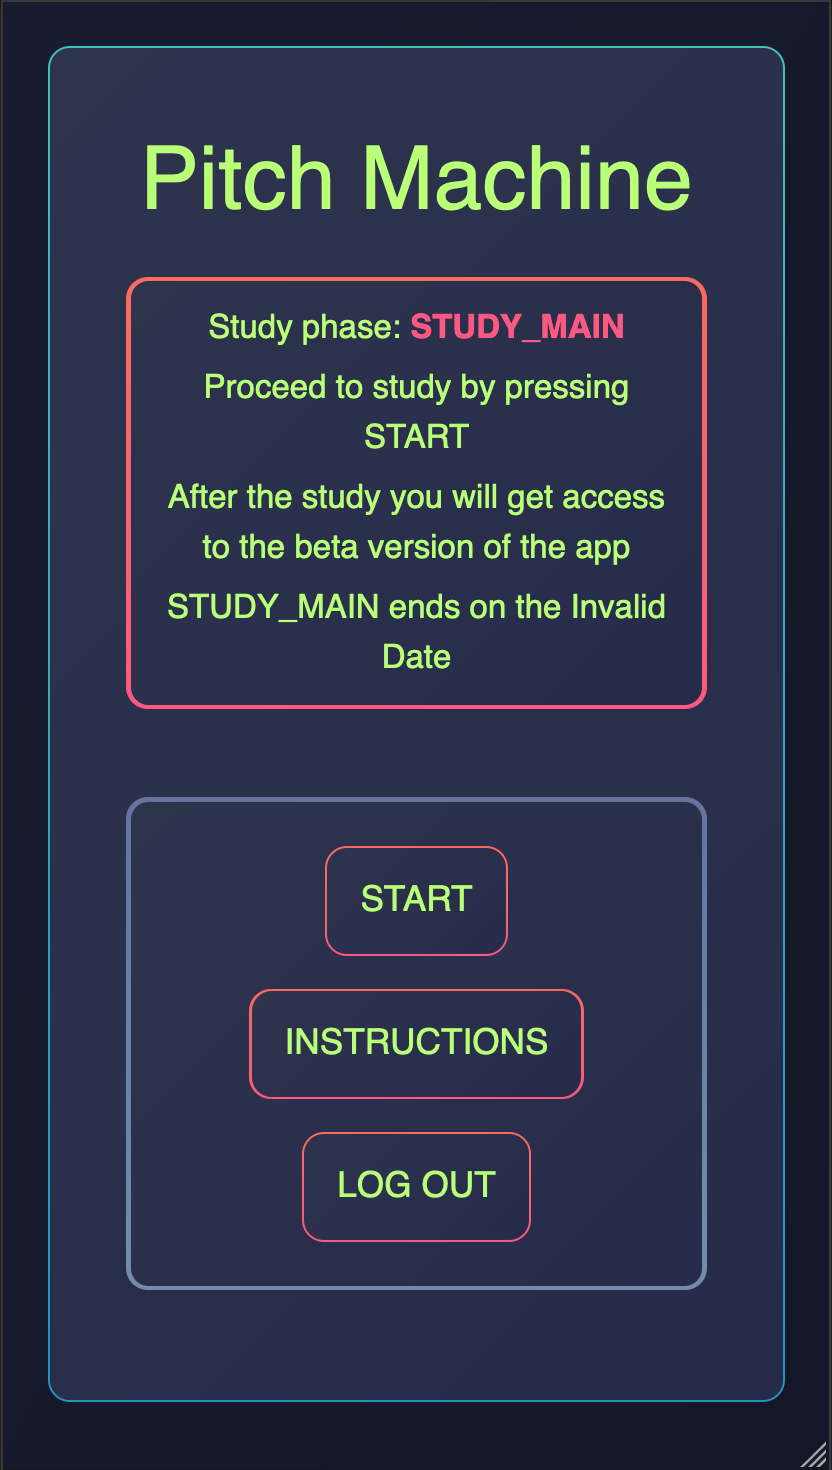
\includegraphics[scale=.33]{Parts/Fig/loggedin.png}
\vspace*{-5mm}
%\textbf{\emph{\caption{\label{fig:intro}introductory screen where particupants have the ability to read about the study and a little bit of music theory.}}}
\end{figure}

\section{Intro screen}
\begin{figure}[H]
\centering
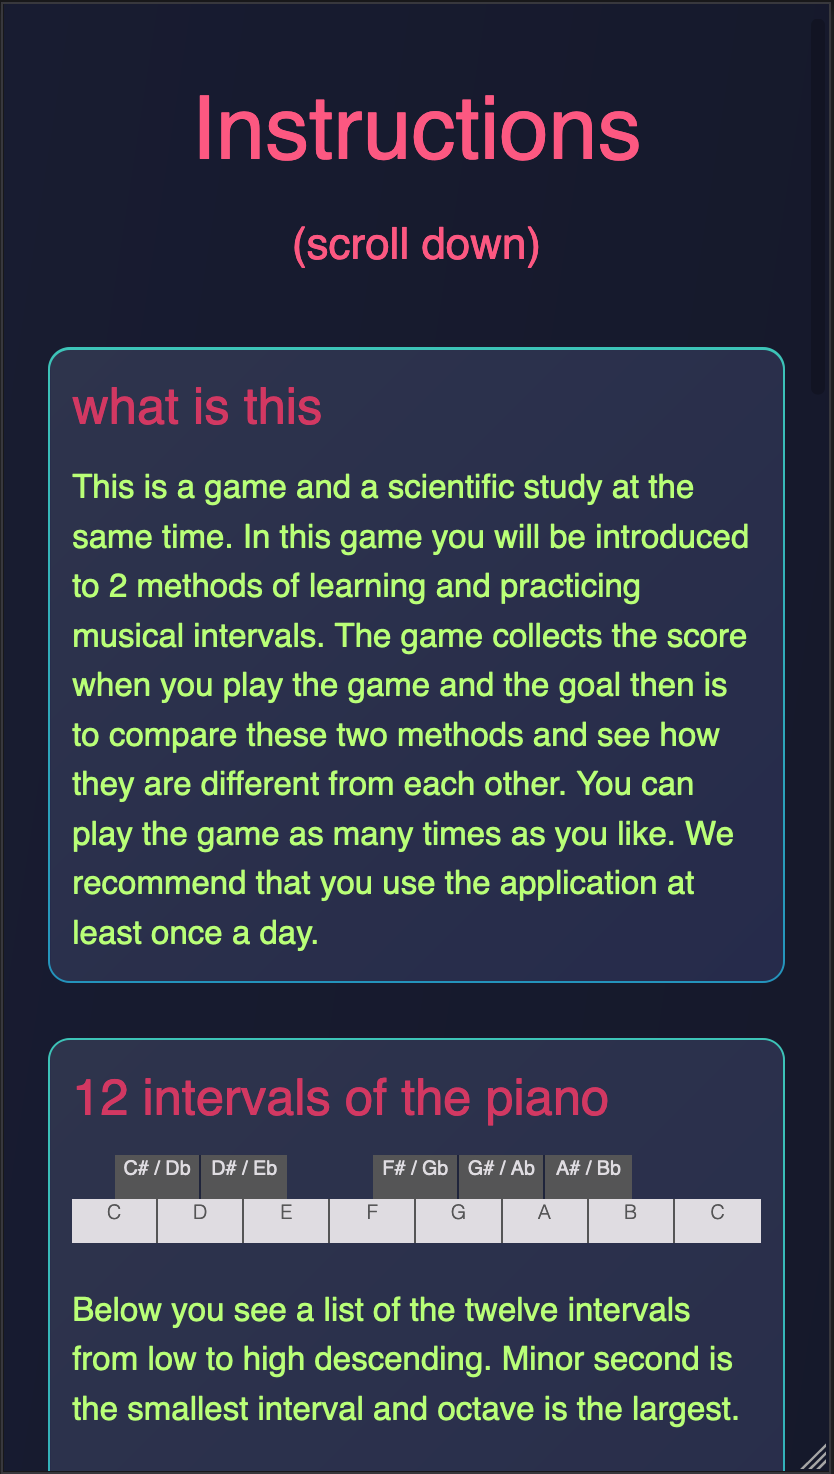
\includegraphics[scale=.33]{Parts/Fig/intro.png}
\vspace*{-5mm}
%\textbf{\emph{\caption{\label{fig:intro}introductory screen where particupants have the ability to read about the study and a little bit of music theory.}}}
\end{figure}


\section{Form}
\begin{figure}[H]
\centering
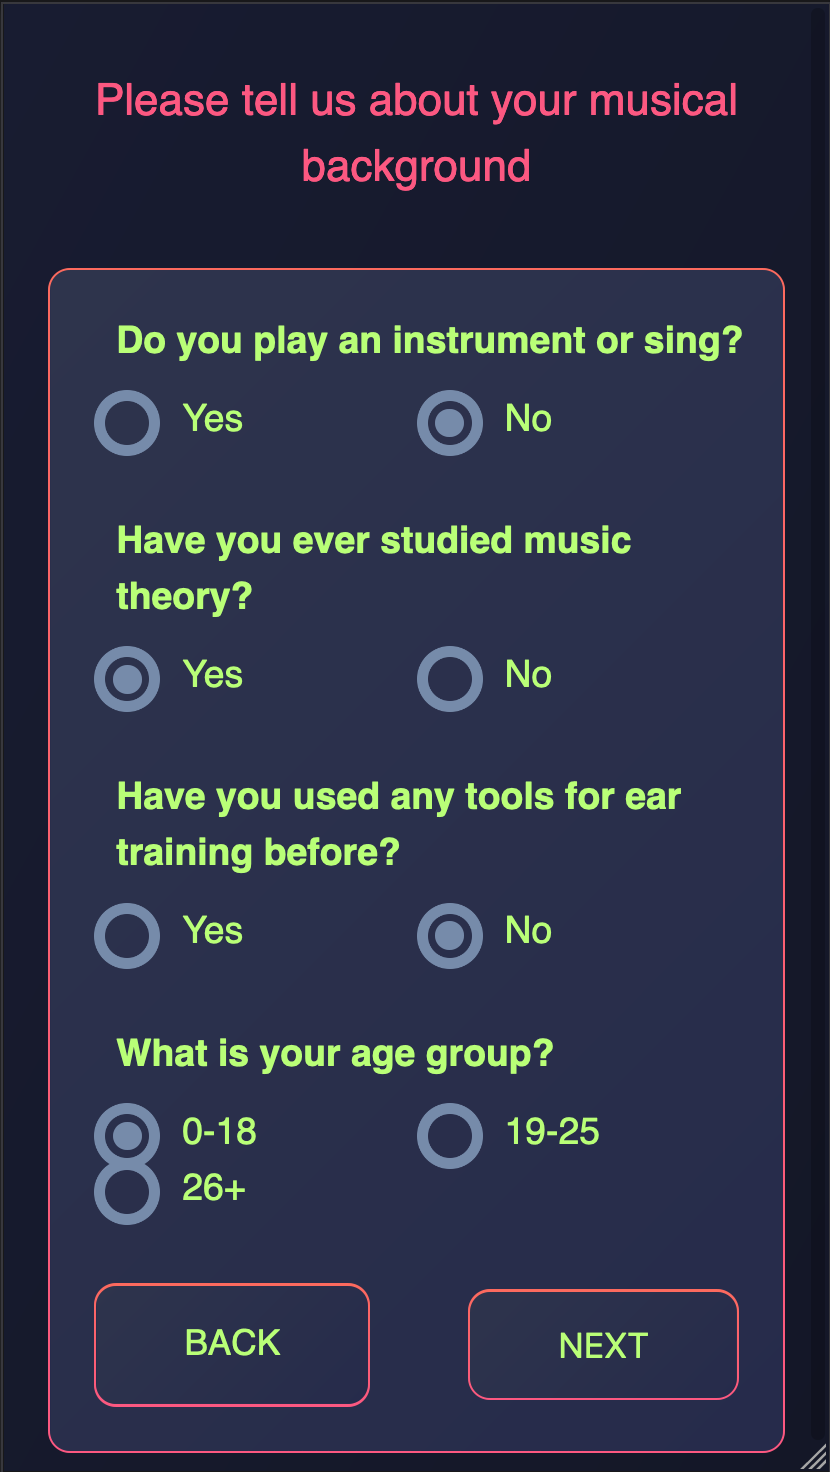
\includegraphics[scale=.33]{Parts/Fig/form.png}
\vspace*{-5mm}
%\textbf{\emph{\caption{\label{fig:intro}introductory screen where particupants have the ability to read about the study and a little bit of music theory.}}}
\end{figure}


\section{Game paused}
\begin{figure}[H]
\centering
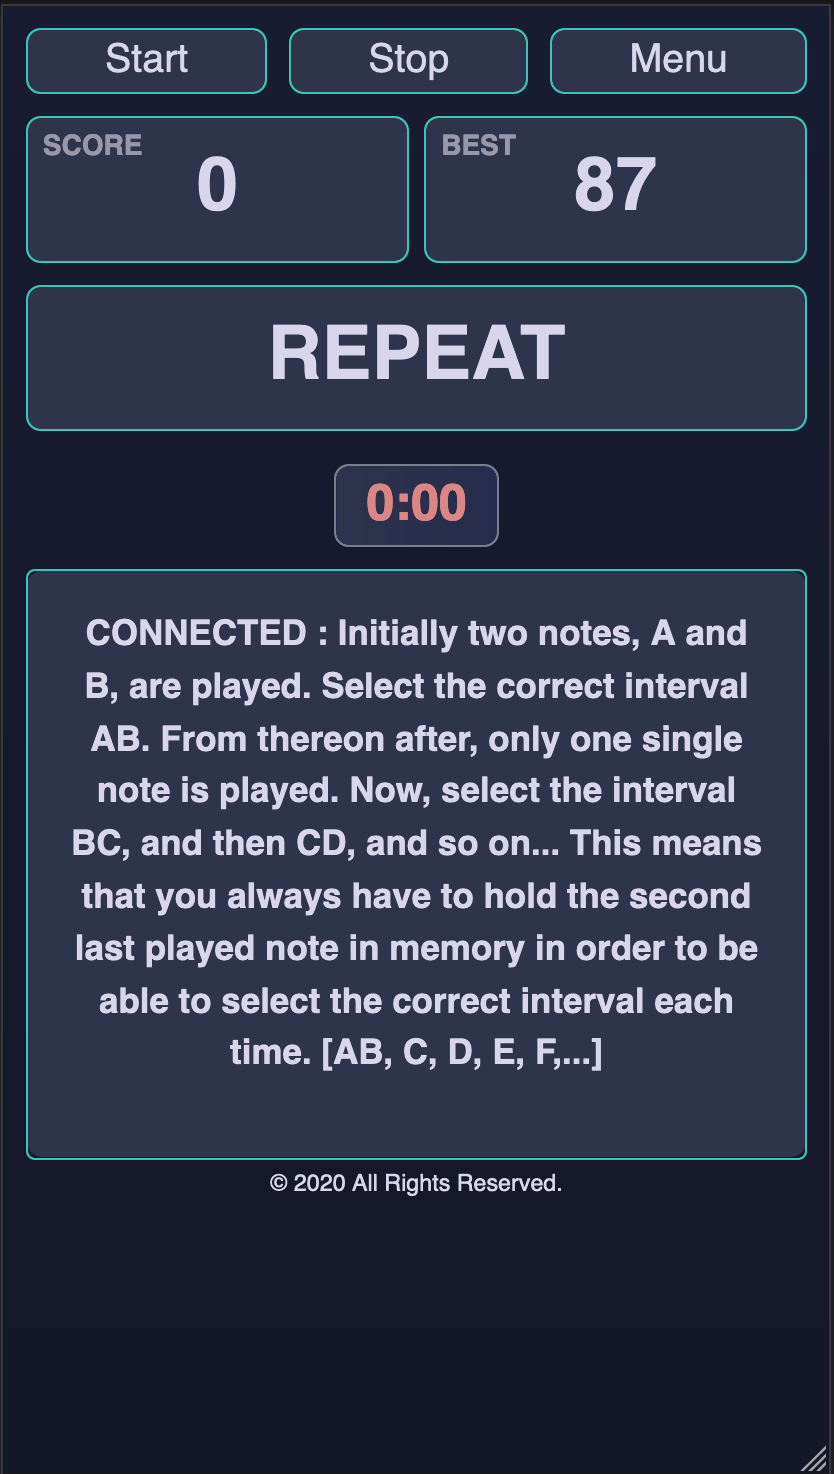
\includegraphics[scale=.33]{Parts/Fig/gamestopped.png}
\vspace*{-5mm}
%\textbf{\emph{\caption{\label{fig:intro}introductory screen where particupants have the ability to read about the study and a little bit of music theory.}}}
\end{figure}


\section{Game playing}
\begin{figure}[H]
\centering
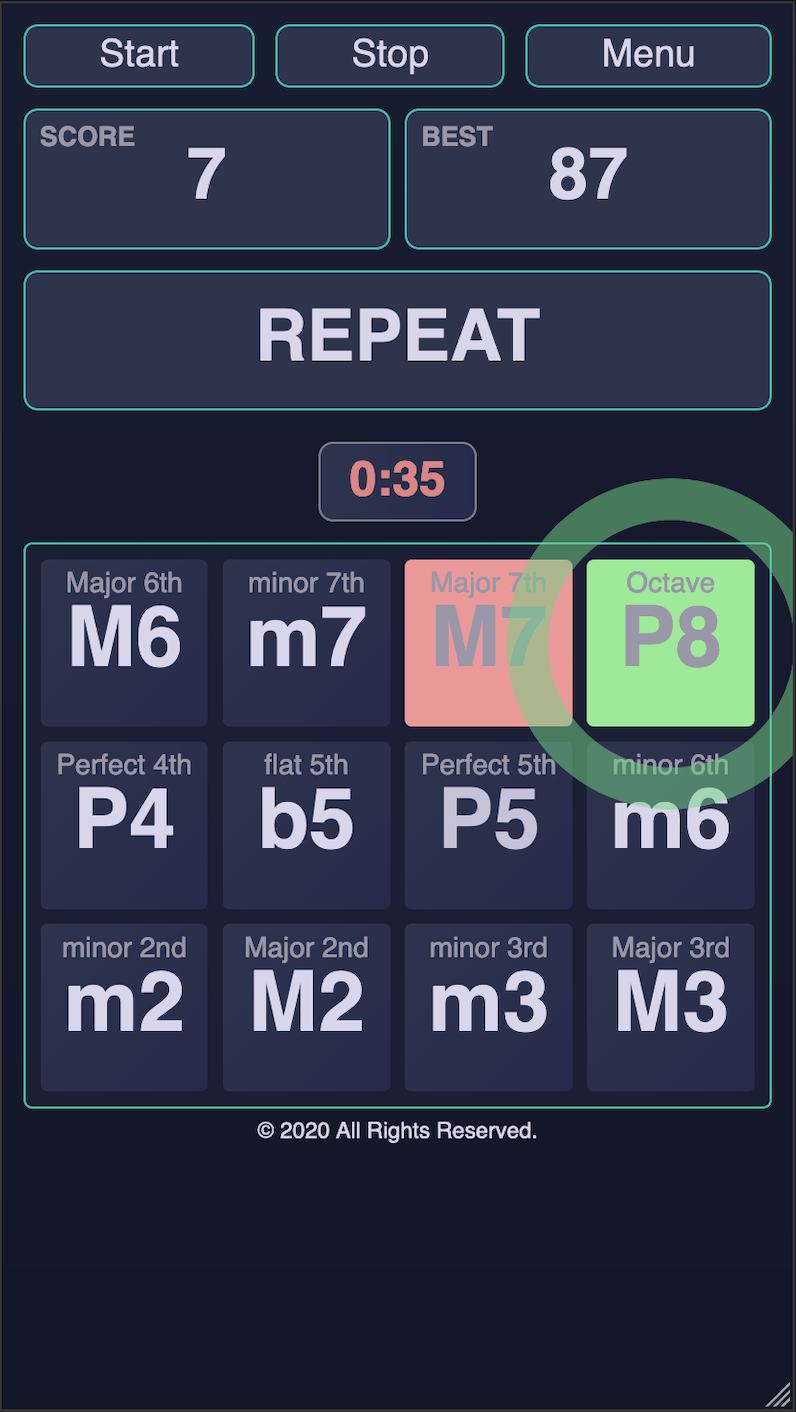
\includegraphics[scale=.33]{Parts/Fig/gameplaying.png}
\vspace*{-5mm}
%\textbf{\emph{\caption{\label{fig:intro}introductory screen where particupants have the ability to read about the study and a little bit of music theory.}}}
\end{figure}

% \begin{figure}[H]
% \centering
% \includegraphics[width=1.1\textwidth]{chapters/Fig/SI2.jpg}
% \vspace*{-5mm}
% \textbf{\emph{\caption{\label{fig:SI2}Algae washed by stirring with acetone.}}}
% \end{figure}
% \begin{figure}[H]
% \centering
% \includegraphics[width=1.1\textwidth]{chapters/Fig/SI3.jpg}
% \vspace*{-5mm}
% \textbf{\emph{\caption{\label{fig:SI3}Algae washed by soxhlet.}}}
% \end{figure}
%
%
% \section{After extraction}
% \begin{figure}[H]
% \centering
% \includegraphics[width=1.1\textwidth]{chapters/Fig/SI1_C.jpg}
% \vspace*{-5mm}
% \textbf{\emph{\caption{\label{fig:SI1_C}The residue from unwashed algae from acid hydrothermal extraction.}}}
% \end{figure}
% \begin{figure}[H]
% \centering
% \includegraphics[width=1.1\textwidth]{chapters/Fig/SI1_CD.jpg}
% \vspace*{-5mm}
% \textbf{\emph{\caption{\label{fig:SI1_CD}The residue from unwashed algae from acid hydrothermal and ultrasonic extraction.}}}
% \end{figure}
% \begin{figure}[H]
% \centering
% \includegraphics[width=1.1\textwidth]{chapters/Fig/SI1_CDE.jpg}
% \vspace*{-5mm}
% \textbf{\emph{\caption{\label{fig:SI1_CDE}Unwashed algae from acid hydrothermal extraction.}}} % $SI1_CDE, Ej SI1_CD$
% \end{figure}
% \begin{figure}[H]
% \centering
% \includegraphics[width=1.1\textwidth]{chapters/Fig/SI1_CE.jpg}
% \vspace*{-5mm}
% \textbf{\emph{\caption{\label{fig:SI1_CE}Unwashed algae from acid hydrothermal extraction.}}}
% \end{figure}
% \begin{figure}[H]
% \centering
% \includegraphics[width=1.1\textwidth]{chapters/Fig/SI1_D.jpg}
% \vspace*{-5mm}
% \textbf{\emph{\caption{\label{fig:SI1_D}The residue from unwashed algae from ultrasonic extraction.}}}
% \end{figure}
% \begin{figure}[H]
% \centering
% \includegraphics[width=1.1\textwidth]{chapters/Fig/SI1_DE.jpg}
% \vspace*{-5mm}
% \textbf{\emph{\caption{\label{fig:SI1_DE}Unwashed algae from ultrasonic extraction.}}}
% \end{figure}
% \begin{figure}[H]
% \centering
% \includegraphics[width=1.1\textwidth]{chapters/Fig/SI2_C.jpg}
% \vspace*{-5mm}
% \textbf{\emph{\caption{\label{fig:SI2_C}The residue from washed algae by stirring with acetone from acid hydrothermal extraction.}}}
% \end{figure}
% \begin{figure}[H]
% \centering
% \includegraphics[width=1.1\textwidth]{chapters/Fig/SI2_CD.jpg}
% \vspace*{-5mm}
% \textbf{\emph{\caption{\label{fig:SI2_CD}The residue from washed algae by stirring with acetone from acid hydrothermal extraction.}}}
% \end{figure}
% \begin{figure}[H]
% \centering
% \includegraphics[width=1.1\textwidth]{chapters/Fig/SI2_CDE.jpg}
% \vspace*{-5mm}
% \textbf{\emph{\caption{\label{fig:SI2_CDE}Washed algae by stirring with acetone from acid hydrothermal and ultrasonic extraction.}}}
% \end{figure}
% \begin{figure}[H]
% \centering
% \includegraphics[width=1.1\textwidth]{chapters/Fig/SI2_CE.jpg}
% \vspace*{-5mm}
% \textbf{\emph{\caption{\label{fig:SI2_CE}Washed algae by stirring with acetone from acid hydrothermal extraction.}}}
% \end{figure}
% \begin{figure}[H]
% \centering
% \includegraphics[width=1.1\textwidth]{chapters/Fig/SI2_D.jpg}
% \vspace*{-5mm}
% \textbf{\emph{\caption{\label{fig:SI2_D}The residue from washed algae by stirring with acetone from ultrasonic extraction.}}}
% \end{figure}
% \begin{figure}[H]
% \centering
% \includegraphics[width=1.1\textwidth]{chapters/Fig/SI2_DE.jpg}
% \vspace*{-5mm}
% \textbf{\emph{\caption{\label{fig:SI2_DE}Washed algae by stirring with acetone from ultrasonic extraction.}}}
% \end{figure}
%

% \chapter{NMR results}
% \label{appB}
%
% The raw data for the NMR results are shown below in \textit{figure \ref{fig:1SI}-\ref{fig:DE_SI2}.}
%
% \section{Before extraction}
%
% \begin{figure}[H]
% \centering
% \includegraphics[width=0.98\textwidth]{chapters/Fig/1SI.jpg}
% \vspace*{-5mm}
% \textbf{\emph{\caption{\label{fig:1SI} Unwashed algae.}}}
% \end{figure}
% \begin{figure}[H]
% \centering
% \includegraphics[width=0.98\textwidth]{chapters/Fig/2SI.jpg}
% \vspace*{-5mm}
% \textbf{\emph{\caption{\label{fig:2SI} Washed algae by stirring with acetone.}}}
% \end{figure}
% \begin{figure}[H]
% \centering
% \includegraphics[width=0.98\textwidth]{chapters/Fig/3SI.jpg}
% \vspace*{-5mm}
% \textbf{\emph{\caption{\label{fig:3SI} Washed algae by soxhlet.}}}
% \end{figure}
%
%
% \section{After extraction}
% \begin{figure}[H]
% \centering
% \includegraphics[width=0.98\textwidth]{chapters/Fig/CE_SI1.jpg}
% \vspace*{-5mm}
% \textbf{\emph{\caption{\label{fig:CE_SI1} Unwashed algae from acid hydrothermal extraction.}}}
% \end{figure}
% \begin{figure}[H]
% \centering
% \includegraphics[width=0.98\textwidth]{chapters/Fig/DE_SI1.jpg}
% \vspace*{-5mm}
% \textbf{\emph{\caption{\label{fig:DE_SI1} Unwashed algae from ultrasonic extraction.}}}
% \end{figure}
% \begin{figure}[H]
% \centering
% \includegraphics[width=0.98\textwidth]{chapters/Fig/DE_SI2.jpg}
% \vspace*{-5mm}
% \textbf{\emph{\caption{\label{fig:DE_SI2} Washed algae by stirring with acetone from ultrasonic extraction.}}}
% \end{figure}

\end{appendices}

% Tailmatter inserts the back cover page (if enabled)
% \tailmatter

\includepdf[pages=2]{kth-cover.pdf}

\end{document}
